\documentclass{article}


% if you need to pass options to natbib, use, e.g.:
%     \PassOptionsToPackage{numbers, compress}{natbib}
% before loading neurips_2022


% ready for submission
%\usepackage{neurips_2022}


% to compile a preprint version, e.g., for submission to arXiv, add add the
% [preprint] option:
%\usepackage[preprint]{neurips_2022}


% to compile a camera-ready version, add the [final] option, e.g.:
\usepackage[final]{neurips_2022}


% to avoid loading the natbib package, add option nonatbib:
%    \usepackage[nonatbib]{neurips_2022}


\usepackage[utf8]{inputenc} % allow utf-8 input
\usepackage[T1]{fontenc}    % use 8-bit T1 fonts
\usepackage[colorlinks]{hyperref}       % hyperlinks
\usepackage{url}            % simple URL typesetting
\usepackage{booktabs}       % professional-quality tables
\usepackage{amsfonts}       % blackboard math symbols
\usepackage{nicefrac}       % compact symbols for 1/2, etc.
\usepackage{microtype}      % microtypography
\usepackage{xcolor}         % colors
\usepackage{amsmath}
\usepackage[english]{babel}
\usepackage[pdftex]{graphicx}
\usepackage{bm}

\newcommand{\argmax}{\arg\max}

\urlstyle{rm}

\bibliographystyle{abbrvnat}

\title{A Decoupled Learning Scheme for the Long-tail Recognition on Image Classification Datasets}


% The \author macro works with any number of authors. There are two commands
% used to separate the names and addresses of multiple authors: \And and \AND.
%
% Using \And between authors leaves it to LaTeX to determine where to break the
% lines. Using \AND forces a line break at that point. So, if LaTeX puts 3 of 4
% authors names on the first line, and the last on the second line, try using
% \AND instead of \And before the third author name.


\author{
  Zeen Chi \\
  School of Information Science and Technology\\
  ShanghaiTech University\\
  Shanghai, China 201210 \\
  \texttt{chize@shanghaitech.edu.cn} \\
  \And
  Zhongxiao Cong \\
  School of Information Science and Technology \\
  ShanghaiTech University\\
  Shanghai, China 201210 \\
  \texttt{congzhx@shanghaitech.edu.cn} \\
}


\begin{document}


\maketitle


\begin{abstract}
    The long-tail distribution of image classification datasets has significantly challenged the existing deep learning based classification models. Many traditional works have proposed various solutions, including re-sampling the training data and modifying the loss function. However, most of the methods are applied by jointly learning the image feature extractor and classifier, which have many disadvantages for long-tail recognition. According to a groundbreaking study in recent years, a surprisingly effective idea is to decouple the learning process into feature representation and classification and train two stages separately. Following the idea, in this article, we apply different sampling and classification methods to the two stages respectively, and systematically conduct experiments for combinations of them on the long-tailed benchmark ImageNet-LT, showing that the disentangled method outperforms the existing sampling strategies and designed losses to some extent. Our code is available at \url{https://github.com/boynextdoor-cze/CS182-Project}.
\end{abstract}


\section{Introduction}

In the past 10 years, as a branch of machine learning and computer vision, image classification research has made significant advances, mainly driven by the appliance of deep convolutional neural networks (CNNs) like ResNet and its improvements \cite{he2016deep, Xie2016} and large-scale real-world datasets like ImageNet \cite{deng2009imagenet}. Most of the datasets are artificially instance-balanced, that is, the numbers of instances in each object class are identical in the training set. However, since data collection costs vary, building a dataset with instance-balanced categories becomes particularly costly, so large-scale image datasets are often class-imbalanced, forming a long-tailed distribution (see Figure \ref{fig1}).

The long-tailed distribution of datasets poses novel and great challenges for traditional image classification techniques. The scarce sample size of the tail categories provides very little information to the neural network model, making it difficult for the model to learn parameters with good generalization performance from the small amount of data. In addition, since the sample size of head categories is at least two orders of magnitude larger than the tail data, the model will focus excessively on fitting head categories, which leads to suppression and insensitivity to the features of tail categories. Therefore, the traditional model trained by the long-tailed datasets will show a serious under-fitting phenomenon to the tail data, resulting in poor overall generalization performance.

To address the issue and improve performance across all classes, one direction is to re-balance the dataset by re-sampling strategies \cite{burnaev2015influence,chawla2002smote,estabrooks2004multiple,huang2016learning,pereira2021toward}, another is to modify loss functions by multiplying weight coefficients \cite{cao2019learning,koziarski2021two,zhang2021mining} or designing new ones \cite{cui2019class,lin2017focal,wang2021adaptive}. A common belief behind the aforementioned methods is that a new sampling strategy or loss function can improve both image feature representation and classification jointly, thus achieving a higher long-tail recognition performance. Nevertheless, applying a strategy alone can make the drawbacks of that strategy magnified, and a scheme in which the two stages are trained together can blur the boundary between feature extraction and classification, making it difficult to distinguish the contribution of the two stages to handling the imbalanced data.

A groundbreaking observation, proposed by Kang \textit{et al.} \cite{kang2019decoupling}, empirically resolved the issue above. According to the observation, the distribution of image features and the distribution of category annotations are, by nature, uncoupled. That means, learning a good image feature extractor is irrelevant to tuning the classification boundaries. Following the key idea, we decouple the long-tail recognition problem into \textit{image representation} and \textit{classification}, then apply a disentangled training scheme to the two stages. In the first stage, we first utilize different class re-sampling strategies and jointly train the feature extractor and classifier, then individually study three different classification approaches after freezing the model parameters of the extractor.

We conduct experiments on the long-tailed image classification dataset ImageNet-LT based on the aforementioned decoupled learning schemes and compare the results of joint ones to disentangled ones on the head, body, and tail parts of the dataset, respectively. In conclusion, we find that the decoupled learning scheme generally outperforms the traditional joint training methods.

The main work of this article is as follows:
\begin{itemize}
    \item We analyze the disadvantages of the existing methods, including re-sampling and re-weighting schemes.
    \item Following the idea of the work Kang \textit{et al.} \cite{kang2019decoupling}, we conduct extensive comparison experiments for a number of combinations of re-sampling and classification strategies on a long-tailed dataset.
    \item We discuss the concrete benefits of decoupled training over joint learning, the key influencing factors for classifiers, and some other interesting observations concluded from experiment results.
\end{itemize}

\begin{figure}
    \centering
    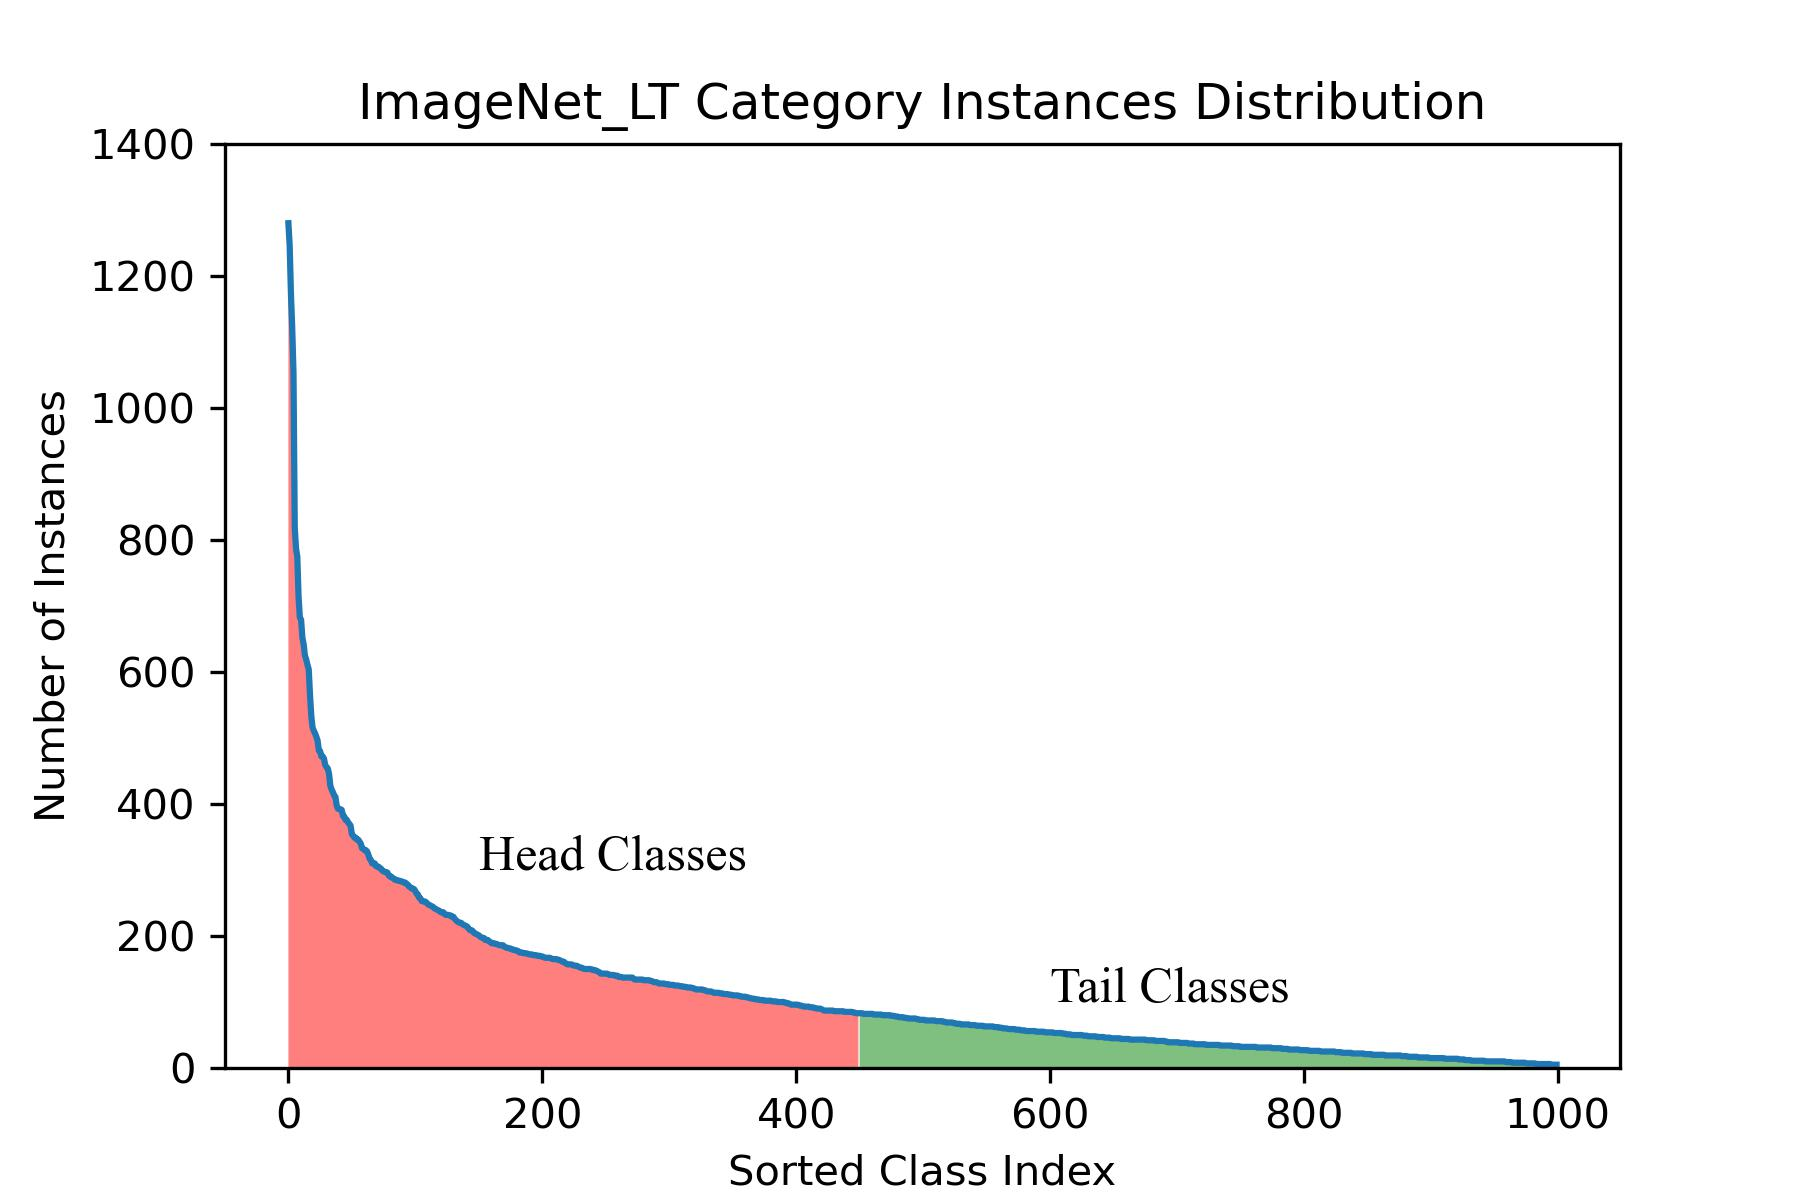
\includegraphics[width=0.6\linewidth]{"report/img/ImageNet_LT.jpg"}
    \caption{The long-tailed distribution on ImageNet-LT dataset. The difference in quantity between head and tail data is noticeably large, often about two orders of magnitude.}
    \label{fig1}
\end{figure}



\section{Related Work}

Most of the previous work about long-tail recognition can be divided into two schemes: re-sampling \cite{burnaev2015influence,chawla2002smote,drummond2003c4,estabrooks2004multiple,han2005borderline,huang2016learning,pereira2021toward} and loss function modifications \cite{cao2019learning,cui2019class,koziarski2021two,lin2017focal,wang2021adaptive,zhang2021mining}. In this section, we will briefly review their main ideas and analyze their flaws.

\paragraph{Re-sampling.}Researchers have come up with some re-sampling strategies for the training data, to achieve a more class-balanced data distribution. The most classical ones are over-sampling for the tail categories \cite{han2005borderline} and under-sampling for the head categories \cite{drummond2003c4}. However, abandoning abundant data impairs the model's excellent generalization ability to the head category, and replicating instances of tail classes causes severe over-fitting to tail classes due to the inadequate sample variance. Fortunately, some techniques like image augmentation, interpolation from neighboring samples \cite{chawla2002smote}, and synthesized novel samples \cite{he2008adaptive,zou2018unsupervised} can help to alleviate the harm.

\paragraph{Loss Function Modifications.}The main idea of loss function modification is to penalize misclassifications on tail classes more heavily for better fitting performance. Some relatively straightforward approaches are assigning weight coefficients with respect to the data distribution to the loss functions. For example, the original cross-entropy loss can be weighted by inverse \cite{huang2016learning,wang2017learning} or inverse squared root \cite{mahajan2018exploring,mikolov2013distributed} of class frequency, Focal Loss \cite{lin2017focal} helps models rapidly focus on hard-to-classify examples by applying scaling factors as a modulating term, and Zhang \textit{et al.} \cite{zhang2021mining} dynamically adjust weights as training progresses. Other mainstream methods directly re-design novel loss functions. Wang \textit{et al.} \cite{wang2021adaptive} adopt adaptive class suppression loss to prevent tail classifiers from being over-suppressed by overwhelming head samples, and Cao \textit{et al.} \cite{cao2019learning} introduce LDAM to allocate larger margin loss and decision boundaries for minority classes. Nevertheless, simply multiplying weights according to class proportions is incapable of handling large-scale real-world long-tailed scenarios, and could unnecessarily allow minority categories to dominate the model \cite{jamal2020rethinking}. Beyond that, most of the existing re-weighting schemes or novel loss functions concentrate more on classification but focus less on the feature representation stage, meaning that the optimization of extracting more representative features on tail categories is difficult to achieve.



\section{Methods}
\subsection{Notation}We first define some notations that will be used in the methods below.

\paragraph{Dataset.} We denote the training set as $\mathcal{X}=\{\mathbf{x}_i,y_i\}_{i=1}^n$, where $\mathbf{x}_i\in\mathbb{R}^{H\times D\times 3}$ is the input image for training, $y_i\in\{1,2,\ldots,C\}$ is the index of category for $\mathbf{x}_i$, $H,D$ are the height and width of each input image, and $C$ is the total number of classes, respectively. Denote $n$ as the total number of training samples and $n_j$ as the number of training samples in $j$-th class (namely cardinality), then $n=\sum_{j=1}^{C} n_j$.

\paragraph{Representation.} Image feature representation is defined by $\mathbf{z}=f(\mathbf{x};\bm{\Theta})$, where $f(\mathbf{x};\bm{\Theta})$ is generally implemented by a deep CNN model with parameter $\bm{\Theta}$, and $\mathbf{z}$ is the extracted feature tensor with respect to the input $\mathbf{x}$.

\paragraph{Classifier.} Let $h$ denote the classification function, into which the image feature $\mathbf{z}$ is fed. Generally, the final class prediction $\hat{y}$ given by $h$ is $\hat{y}=\argmax h(\mathbf
{z})$. Some modern techniques adopt a single-layer linear classifier or multi-layer perceptron (MLP) followed by a softmax function as the classifier, which can be reduced to $h(\mathbf{z})=\mathrm{softmax}\left[\mathbf{W}_1\sigma(\mathbf{W}_2\sigma(\cdots)+\mathbf{b}_2)+\mathbf{b}_1\right]$ with arbitrary nested level, where $\mathbf{W},\mathbf{b}$ are weights and biases, and $\sigma$ is the activation function (sigmoid, ReLU, etc.), respectively.

\subsection{Image Representation}


% For the long-tailed distribution problem, the training set is not evenly distributed, because the head classes have more instances and dominate the training process. As a result, the learned model tends to exhibit under-fitting on the tail (instance-scarce) classes.
To alleviate the harm of the long-tailed distribution of the training set, in this section we utilize four different sampling strategies to re-balance the distribution of the data for the image feature representation stage.

The probability of sampling a data point from class $j$ in these four sampling methods can be reduced to the following general formula:
\begin{equation}
    p_j=\frac{n_j^{q}}{\sum_{i=1}^{C}n_i^{q}}
\end{equation}
where $q\in[0,1]$ will be set differently according to the specific sampling strategy.

\paragraph{Instance-balanced sampling.}As the most straightforward method, we randomly grab data from the dataset and the probability of each class being sampled is proportional to the category cardinality $n_j$, i.e., $q=1$, so the probability that each sampled data belongs to class $j$ is $p_j^{\mathrm{IB}}=\frac{n_j}{\sum_{i=1}^{C}n_i}$.

\paragraph{Class-balanced sampling.}In this method, each class can be sampled with equal probability, i.e., $q=0$, so the probability of each sampled data belonging to class $j$ is $p_j^{\mathrm{CB}}=1/C$, thus making each class occur with equal probability. This approach solves the problem of under-fitting for few-shot classes caused by instance-balanced sampling.

\paragraph{Square-root sampling.}We set $q=1/2$ in square-root sampling \cite{mikolov2013distributed}. The square root can mitigate the unevenness of the distribution, which serves as a compromise between instance-balanced sampling and class-balanced sampling.

\paragraph{Progressively-balanced sampling.} This is a combination of the first two sampling methods. At the beginning of training, we utilize instance-balanced sampling, but as the training epoch increases, we gradually shift instance-balanced sampling to class-balanced sampling by progressively interpolating the former and the latter based on the training epoch. According to equation \ref{eq2}, suppose the total training epoch is $N$ and the current epoch is $n$, we give the probability of each sampled data being in class $j$ as:
\begin{equation}
    p_j(n)=(1-\frac{n}{N})p_j^{\mathrm{IB}}+\frac{n}{N}p_j^{\mathrm{CB}}
    \label{eq2}
\end{equation}


\subsection{Classification}

In this section, we follow the two-stage decoupled scheme to train the classifier. After training the image feature representation stage, we should freeze the parameters of the backbone, then execute the whole training process again for epochs to separately train the classifier, i.e., rectify the classification decision boundaries on the head and tail classes. We either apply different adjustments to the existing classifier or utilize non-parametric methods to achieve better classification effects.

\paragraph{Classifier Re-training (cRT).}This approach uses a linear classifier $g$ with weights $\mathbf{W}$ and biases $\mathbf{b}$, and randomly initializes them in the beginning. After finishing the image representation stage, we should freeze the parameters of the feature extractor during classifier learning. We feed the input data to the fixed feature extractor (the CNN-based backbone), then pass it through the classifier, updating the classifier parameters $\mathbf{W}$ and $\mathbf{b}$ according to the loss.

\paragraph{Nearest Class Mean classifier (NCM).}In contrast to the softmax classifier where a weight vector is learned for each class, in NCM, the class representation is solely based on the mean representation of the images belonging to that class. The adopted method is to first calculate the mean feature representation of each class on the training set, and then calculate pair-wise class similarities by either $L_2$-norm or cosine similarity \cite{guerriero2018deepncm}. For an input image, we classify it to the class with the closest distance \cite{rebuffi2017icarl,snell2017prototypical}.

\paragraph{$\tau$-normalized classifier ($\tau$-normalized).}Another approach is to directly change the weights $\mathbf{W}$ in the classifier training stage. Denote $w_j$ as the weight of class $j$ that we learned in the classifier, $w_j$ is scaled by
\begin{align}
    \hat{w}_j=\frac{w_j}{||w_j||^{\tau}}
\end{align}
where $||\cdot||$ is the $L_2$ norm and $\tau\in [0,1]$ is a hyper-parameter which controls the degree of scaling \cite{kang2019decoupling}. This method is based on the observation that when joining image representation and classifier learning under different sampling methods, $||w_j||$ is correlated with the cardinality of class $j$. Specifically, under instance-balanced sampling, $||w_j||$ is proportional to the cardinality, while under class-balanced sampling, $||w_j||$ tends to be consistent (see Figure \ref{fig2}).
\begin{figure}
    \centering
    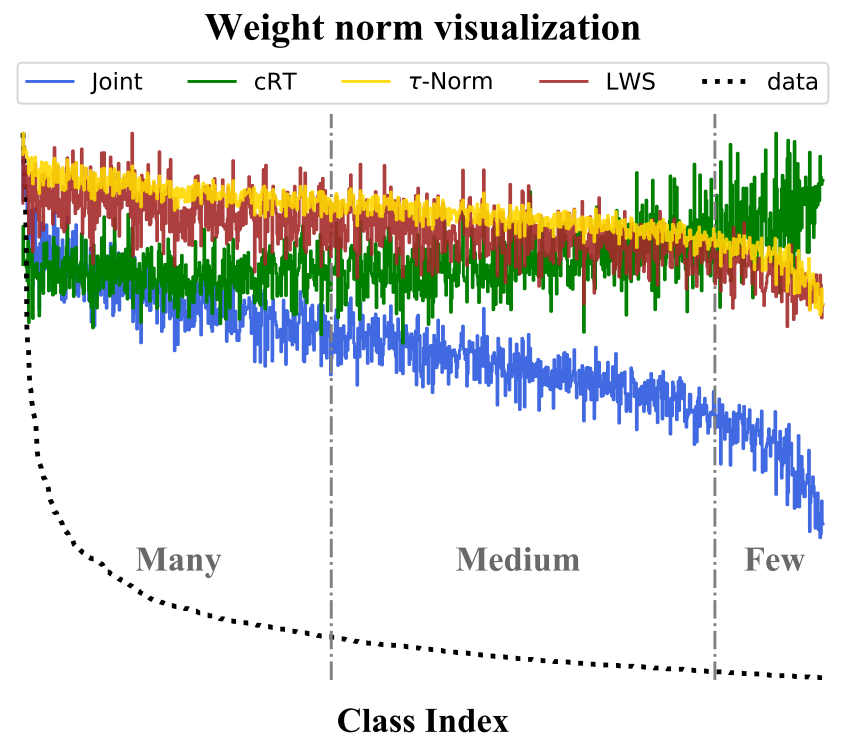
\includegraphics[width=0.5\textwidth]{../img/weights_of_diff_sample.png}
    \caption{Classifier weight norms for ImageNet-LT validation set when classes are sorted by descending values of $n_j$. Blue line: classifier weights learned with instance-balanced sampling. Green line: weights after fine-tuning with class-balanced sampling. Gold line: after $\tau$ normalization. Brown line: weights by learnable weight scaling. The figure comes from \cite{kang2019decoupling}.}
    \label{fig2}
\end{figure}

\section{Experiments}

\subsection{Experimental settings}

\paragraph{Datasets.}We utilize the imbalanced dataset ImageNet-LT \cite{liu2019large} in our experiment which is a long-tailed subset of the large-scale real-world dataset ILSVRC-2012 (ImageNet) \cite{deng2009imagenet}. The class with the maximum number of images contains 1,280 examples, whereas the class with the minimum number of images contains only 5, just like what is shown in Figure \ref{fig1}. The validation and testing sets are class-balanced, which are also subsets of the ILSVRC-2012 training set and contain 20 images per class.

\paragraph{Implementation.}We utilize the PyTorch \cite{NEURIPS2019_bdbca288} framework to build the network. For most general cases, we use SGD optimizer which has a learning rate of 0.2 with a weight decay of 0.0005, batch size of 512, and momentum set to 0.9. In the two stages of learning, we use different numbers of training epochs separately. When learning the representation, we utilize ResNeXt-50 \cite{Xie2016} as the backbone, which has been pretrained on the full ImageNet dataset, and train the network for 90 epochs; when learning the classifier, we train the network for 10 epochs \cite{kang2019decoupling}. For $\tau$-normalization, we set the hyperparameter $\tau=0.9$.

\paragraph{Evaluation.}The model is expected to perform well with generalization over each category---both major classes and minor classes. Therefore, a reasonable evaluation metric is to calculate the accuracy of each category on the validation or test set and then average it. In order to clearly represent the improvement of the effect of different methods on the sparse categories, following Kang \textit{et al.} \cite{kang2019decoupling}, we divide the data into three parts according to the cardinality of each category: \textit{Many-shot}, \textit{Medium-shot} and \textit{Few-shot}. If the cardinality of a category is greater than 100, it is classified into the \textit{Many-shot}; if it is less than 20, it is classified into the \textit{Few-shot}; and the rest is classified into the \textit{Medium-shot}. 


\subsection{Experiment Methods}

For representation learning, other than instance-balanced sampling (instance), the most straightforward and typical sampling strategy, we also adopt class-balanced sampling (class), square-root sampling (square), and progressively-balanced sampling (progressive) respectively. For classification learning, in spite of the traditional one-stage method (Joint), we apply classifier re-training (cRT), nearest class mean classifier (NCM), and $\tau$-normalized classifier (Tau) respectively as different schemes to refine the classification stage. As shown in Figure \ref{fig3}, we combine the two stages pair-wisely and conduct extensive experiments for each combination on the \textit{Many-shot}, \textit{Medium-shot}, and \textit{Few-shot} parts of ImageNet-LT dataset respectively, and evaluate the overall accuracy on all categories.

\begin{figure}[t]
    \centering
    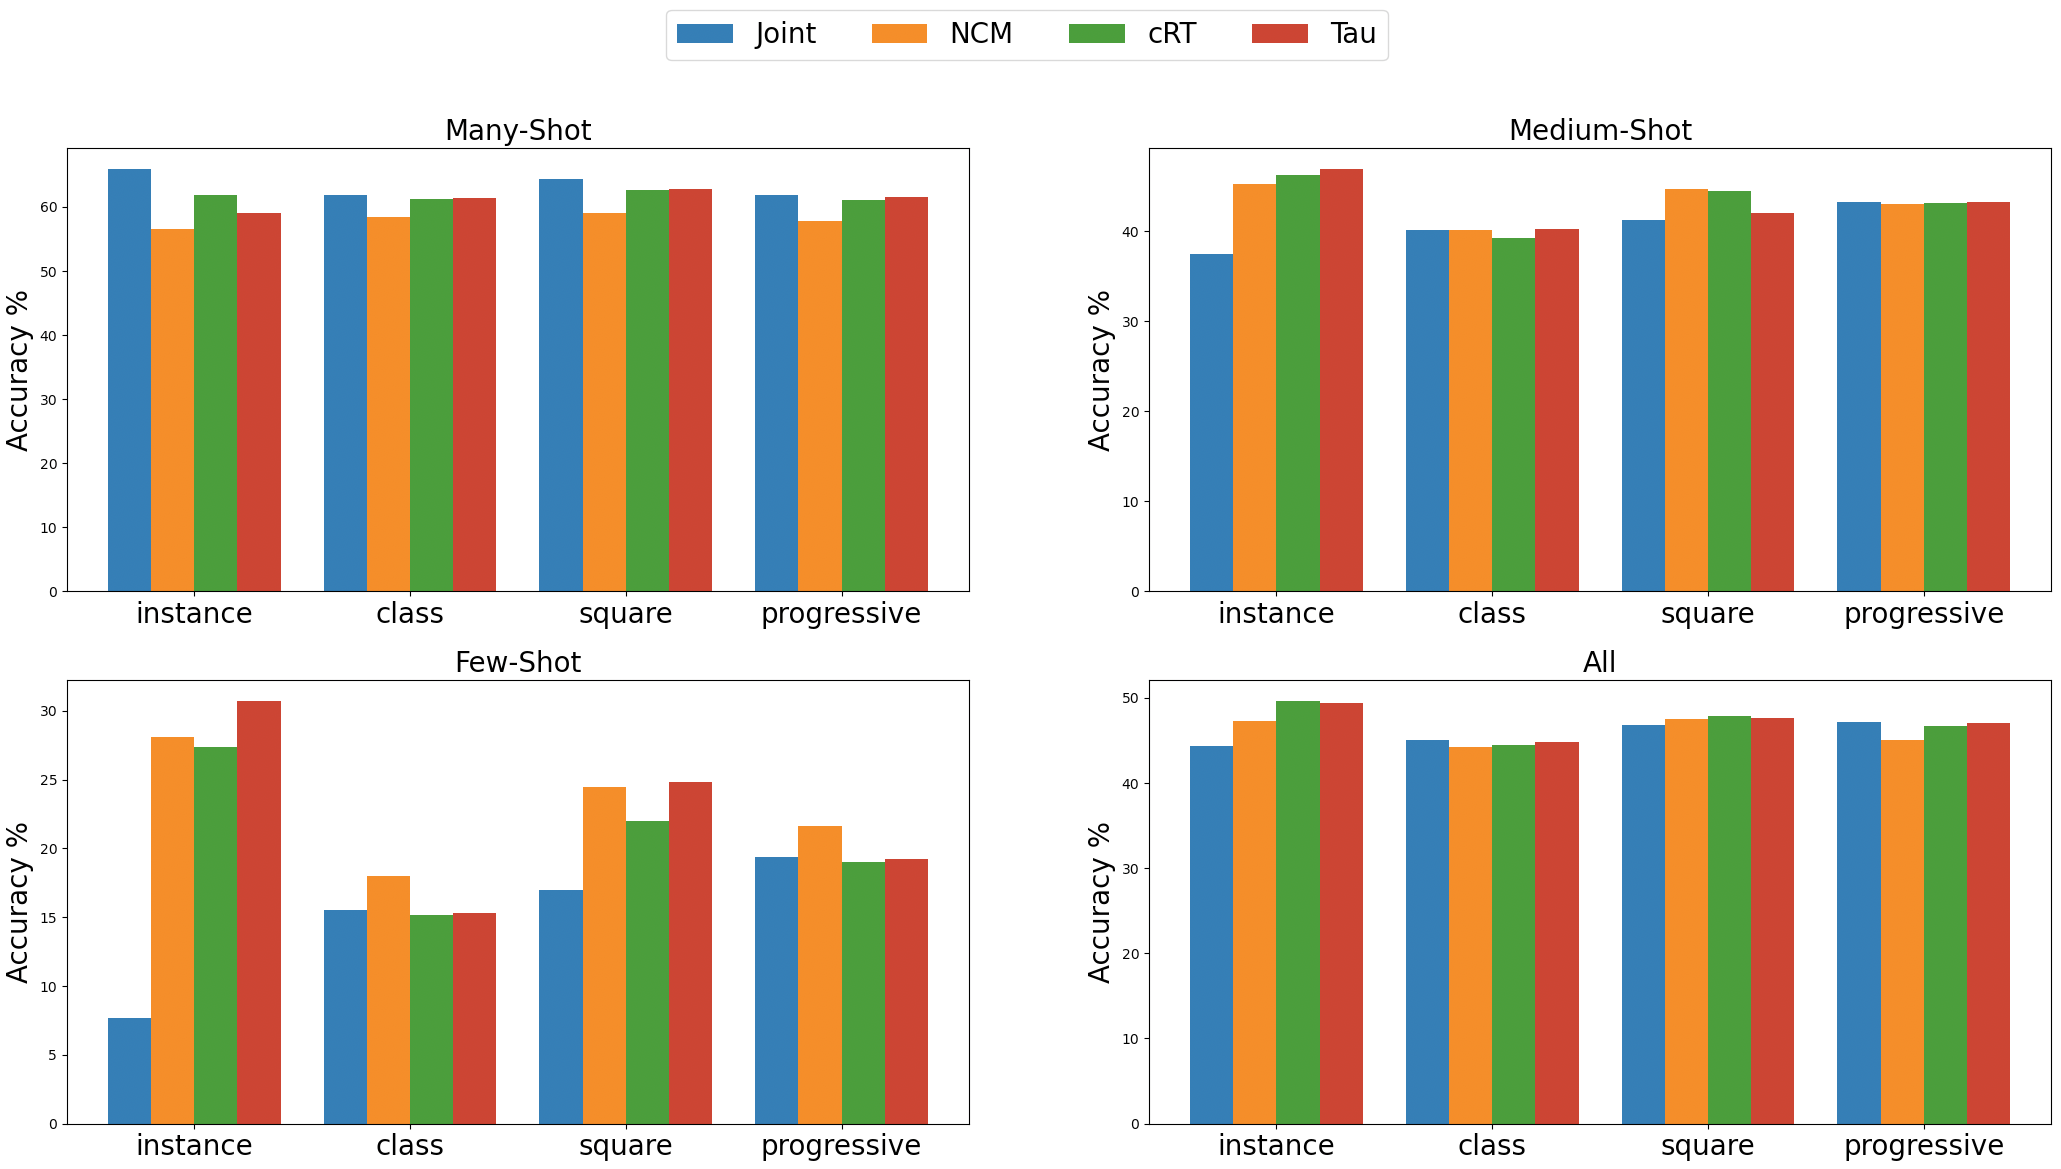
\includegraphics[width=\textwidth]{report/img/result.png}
    \caption{The performance of difference decoupling training scheme with backbone ResNeXt-50 on different parts of dataset ImageNet-LT.}
    \label{fig3}
\end{figure}

\begin{table}
    \caption{Few-shot scenario accuracy for different combinations}
    \label{tab1}
    \centering
    \begin{tabular}{lcccc}
    \toprule
    Classifier     & Instance  & Class & Square & Progressive \\
    \midrule
    Joint          & 7.7       & 15.5  & 17.0   & 19.4        \\
    NCM            & 28.1      & \textbf{18.0}  & 24.5   & \textbf{21.6}        \\
    cRT            & 27.4      & 15.2  & 22.0   & 19.0        \\
    Tau            & \textbf{30.7}      & 15.3  & \textbf{24.8}   & 19.2        \\
    \bottomrule
    \end{tabular}
    \quad
    \caption{Overall accuracy for different combinations}
    \label{tab2}
    \centering
    \begin{tabular}{lcccc}
    \toprule
    Classifier     & Instance  & Class & Square & Progressive \\
    \midrule
    Joint          & 44.4       & 45.1  & 46.8   & 47.2       \\
    NCM            & 47.3      & 44.2  & 47.5   & 45.1        \\
    cRT            & \textbf{49.6}      & 44.5  & \textbf{47.9}   & 46.7        \\
    Tau            & 49.4      & \textbf{45.2}  & 47.6   & \textbf{47.5}        \\
    \bottomrule
    \end{tabular}
\end{table}


\subsection{Results and Analysis}

Based on the results of Figure \ref{fig3}, we would elaborate on our key observations and briefly analyze them.

\paragraph{Decoupled learning outperforms joint learning.}For most cases shown in Figure \ref{fig3}, especially for the few-shot scenario, the decoupled learning schemes significantly surpass the joint learning method by a large margin. Table \ref{tab1} specifically shows different learning schemes combinations on the few-show scenario, and we see that decoupled learning like NCM and $\tau$-normalization achieve at least 3\% improvement compared to the joint learning baseline, and the gains are even higher on instance-balanced sampling strategy, which are over 20\%, even having a 10\% improvement compared with the best sampling strategy (progressively-balanced) for joint learning. For overall accuracy shown by Table \ref{tab2}, benefiting from the better generalization performance on tail classes, the overall accuracy of decoupled learning also has a slight advantage over joint learning.

\paragraph{Instance-balanced sampling generalizes the best.}Comparing difference sampling strategies for decoupled learning methods, we find that when applying instance-balanced sampling, on average and in each of the three cases, the accuracy rate is relatively the highest. Here we have an interesting observation: the imbalance of data distribution might not be a negative factor for high-quality image feature extraction.

\paragraph{Classifiers with more balanced weights perform better.}According to the results, the accuracy of cRT and $\tau$-normalization are generally better than that of NCM. That is because, as shown in Figure \ref{fig2}, $\tau$-normalization (gold line) alleviates the trend that fewer-shot classes tend to have a smaller weight norm as shown by the blue line, and cRT (green line) achieves a more balanced weight norm distribution and even a higher magnitude on tail classes. This amelioration helps a lot when classifying tail categories by preventing them from being suppressed by head classes in terms of the decision boundaries. Such adaptation of weight magnitudes would perform better than NCM, whose weight norms are identical due to the $L_2$ normalization.

\section{Conclusions}

In this work, we compare a number of combinations of decoupled learning schemes of the long-tail recognition to the traditional joint learning method by conducting extensive experiments on the long-tailed dataset ImageNet-LT. We find that the imbalance of data distribution may not be a negative factor of high-quality representation learning because instance-balanced sampling generally performs the best. More importantly, disentangling the training process into image representation and classification significantly alleviates the low accuracy of tail categories. That means we can still achieve a relatively higher classification accuracy without carefully designing the sampling strategies or loss functions. We believe that the decoupled observation can serve as an inspiration, assisting future work to adopt this idea to optimize their training schemes.


{
\small

\bibliography{ref}
}


\end{document}